% arara: closepdf
% arara: pdflatex
% arara: convert: {density: 160, otheroptions: -dispose previous -delay 15 -loop 1, format: gif}
% arara: showfile: {format: gif}
\documentclass{article}
\usepackage[utf8]{inputenc} %probably not needed ...
\usepackage[T1]{fontenc}
\usepackage{geometry}
\geometry{papersize={128mm,96mm},margin=0.5cm} %\textwidth=11.8, \textheight=8.6
\usepackage[x11names,svgnames]{xcolor}
\usepackage{eso-pic}
\usepackage{tikzducks}
\pagestyle{empty}
\newcommand{\myframe}{\draw[white] (-7,-3) rectangle (4,5);}
\newcommand{\frenchduck}{\begin{scope}[scale=.5]
	\clip (0,0) -- ++(2.2,0) -- ++(0,2.6) -- ++(-2.2,0) -- cycle;	
	\duck[body=yellow!60!red!30!white,tshirt=white!90!
	yellow,stripes={\stripes[color=blue!70!black,rotate
		=-87,width=0.07,distance=0.12]},beret=blue!30!black
	,baguette=brown]
	\end{scope}}

\begin{document}
	\AddToShipoutPictureBG{%
		\AtPageLowerLeft{%
			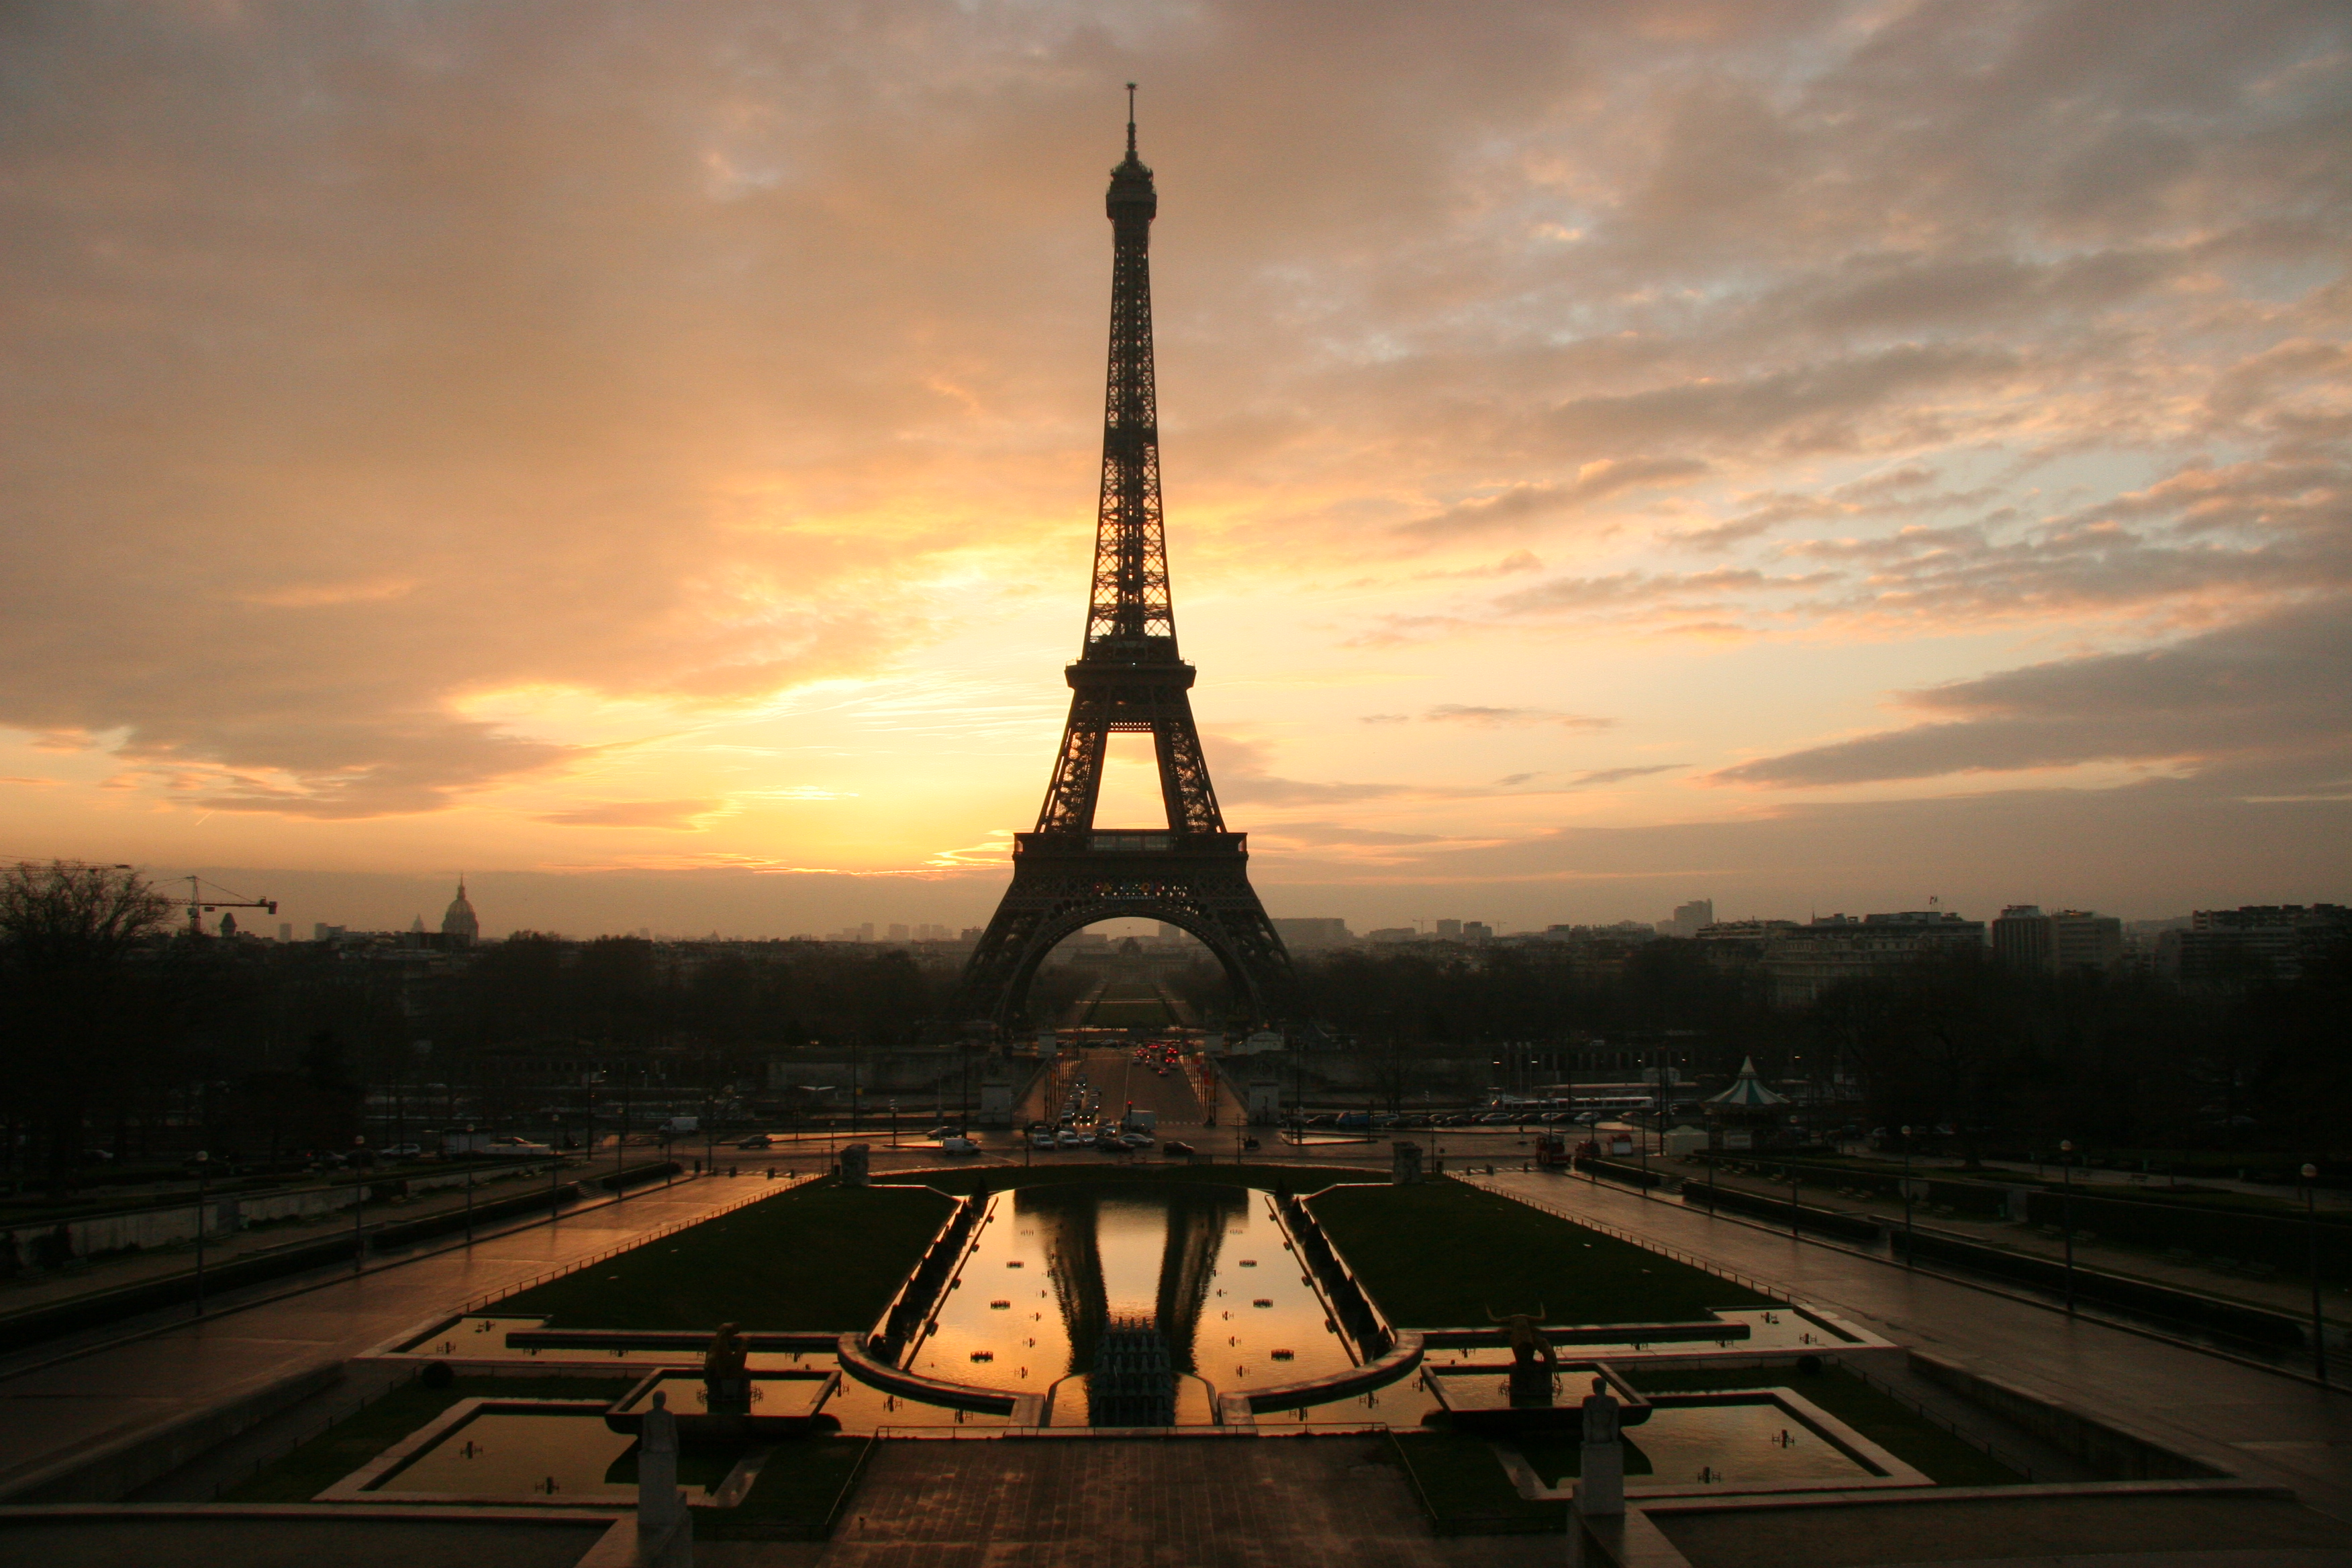
\includegraphics[trim=3cm 0cm 0cm 0cm,height=\paperheight]{EiffelTower.jpg}%
	}}
	\begin{figure}
	\centering
	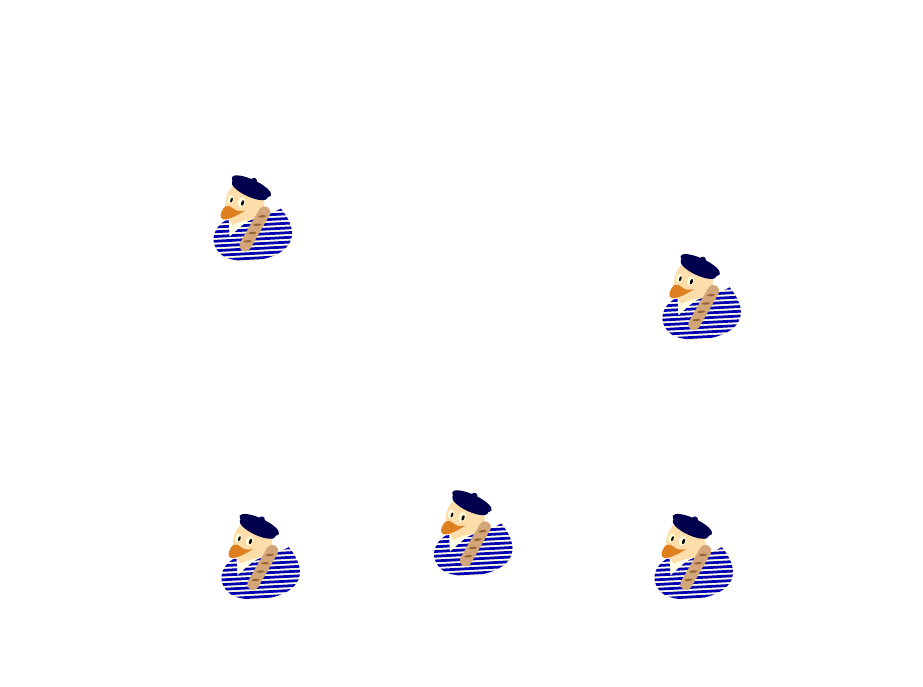
\begin{tikzpicture}
		\myframe
		\foreach \x/\y in {-4.6/-2.3,-1.9/-2,.9/-2.3, -4.7/2,1/1 } {%
			\begin{scope}[shift={(\x, \y)}]
			\frenchduck
			\end{scope}
		}
	\end{tikzpicture}	
	\end{figure}
	\begin{figure}
		\centering
		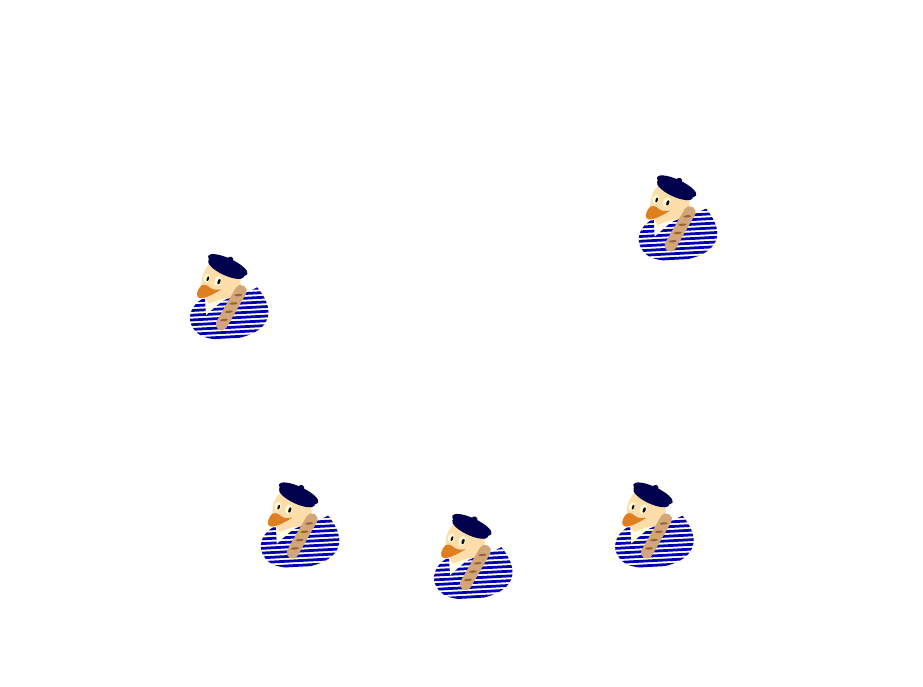
\begin{tikzpicture}
		\myframe
		\foreach \x/\y in {-4.1/-1.9,-1.9/-2.3,.4/-1.9, -5/1,.7/2 } {%
			\begin{scope}[shift={(\x, \y)}]
			\frenchduck
			\end{scope}
		}
		\end{tikzpicture}	
	\end{figure}
\end{document}
